%%%%%%%%%%%%%%%%%%%%%%%%%%%%%%%%%%%%%%%%%%%%
\section{Future of Collaboration}\label{sec:future}
%%%%%%%%%%%%%%%%%%%%%%%%%%%%%%%%%%%%%%%%%%%%


\padis and \cate are designed to enable cooperation between CDI and ISPs for
the already deployed servers. Recent advances in virtualization offer CDIs
additional degree of freedom to scale-up or shrink the footprint on demand.
This can be done either by jointly deploying and operating new servers with the
ISPs.  In this section we formally introduce the design of on-demand services
motivated by the recent announcement of major ISPs to support generic
hardware-network appliances, also referred to as microdatacenters, and offer
them to application, service, and content providers. We also provide the design
and implementation of \Netpaas, a system to orchestrate the deployment of
on-demand services inside microdatacenters, by utilizing the view of the ISP
about the network and additional computation and storage resources inside the
network.

\subsection{The New Cloud: Microdatacenters Deep Inside the Network}\label{sec:generic-appliances}

Applications are increasingly relying on direct interactions with end-users and
are very sensitive to delay~\cite{ImprovingPerformanceInternet2009}. Indeed,
transaction delay is critical for online
businesses~\cite{amazon-study-about-transaction-speed}.  Network delay and loss
are important contributors.  Today, large-scale service deployments are
restricted by limited locations in the network, \eg datacenters, peering
locations, or IXPs. These locations are not necessarily ideal~\cite{CloudCmp}.
We point out that \emph{selection of service location is critical and currently
not flexible enough}.  Services should be located close enough to, in terms of
network distance, the clients.  Since client demands are volatile and change
across time, CDIs need agility~\cite{EmbrassingleDistributed}.  They can
improve their service quality by quickly allocating, de-allocating, and
migrating resources on-demand where and when they are needed. Indeed, since
delay and packet loss are among the critical metrics, the service may need to
be deployed deep inside the network, as many ISPs do for IPTV services. This
option is not yet available for non-ISP content delivery Infrastructures, \eg
for cloud services.

Currently, most services and networks are run by independent entities with
different and often conflicting objectives. Lack of information about the other
entity leads to suboptimal performance and resource allocation for both the CDI
and the ISP. For example, CDIs implement sophisticated methods to infer network
conditions to improve perceived end-user experience~\cite{Akamai-Network}, \eg
active measurements within the ISPs. Yet, the information gleaned from these
measurements is already available with far greater precision to the ISP. On the
other hand, ISPs continuously upgrade their infrastructures without being able
to efficiently engineer the CDI traffic flows~\cite{PADIS2010}. Today,
cooperation and/or partnership between providers is limited to, \eg peering or
lately direct interconnections with content delivery Infrastructures. This
level of cooperation is too narrow to reduce operational costs, improve
end-user experience, circumvent bottlenecks, handle flash crowds, and adapt to
changing network conditions and user demands. This has led to initial
discussions on how to improve communication between the various entities, \eg
within the IETF ALTO and CDNi working groups.


\subsubsection{The ISPs Proposal}\label{NFV}

To overcome the above mentioned obstacles in service deployment and operation,
major ISPs, including AT\&T, Verizon, Deutsche Telekom, Telefonica, NTT, have proposed
the use of cloud resources consisting of general purpose appliances that are
co-located at network aggregation points inside the ISP. With the convergence
of computing, storage, and communications, the acceptance of cloud services,
and the ever increasing demand for popular services, ISPs are moving towards
deploying general-purpose computing and storage infrastructures in their points
of presences (PoPs). Henceforth, we refer to these as \emph{microdatacenters}.
The description of the functionality of these microdatacenters is provided in a
white paper~\cite{NFV} that appeared in the SDN and OpenFlow World Congress in
October 2012 and signed by 13 of the largest ISPs. Microdatacenters can be also
the technical solution needed to materialize recent alliances of major CDIs,
such as Akamai with large ISPs in the area of content
delivery~\cite{content-delivery-alliance1,content-delivery-alliance2,content-delivery-alliance3}.
We notice that Software Defined Networks (SDNs) is another alternative to
redirect traffic or perform traffic engineering when applied within an ISP or
between and ISP and a CDN in cooperation.  The comparison of the two
approaches, NFV and SND, is out of the scope of this chapter and we refer the
users to the related literature on SDN
\eg~\cite{Ethane,NOX,OpenFlow,SDN-Internet-Infrastructure,B4}.

\begin{figure} 
\begin{center}
	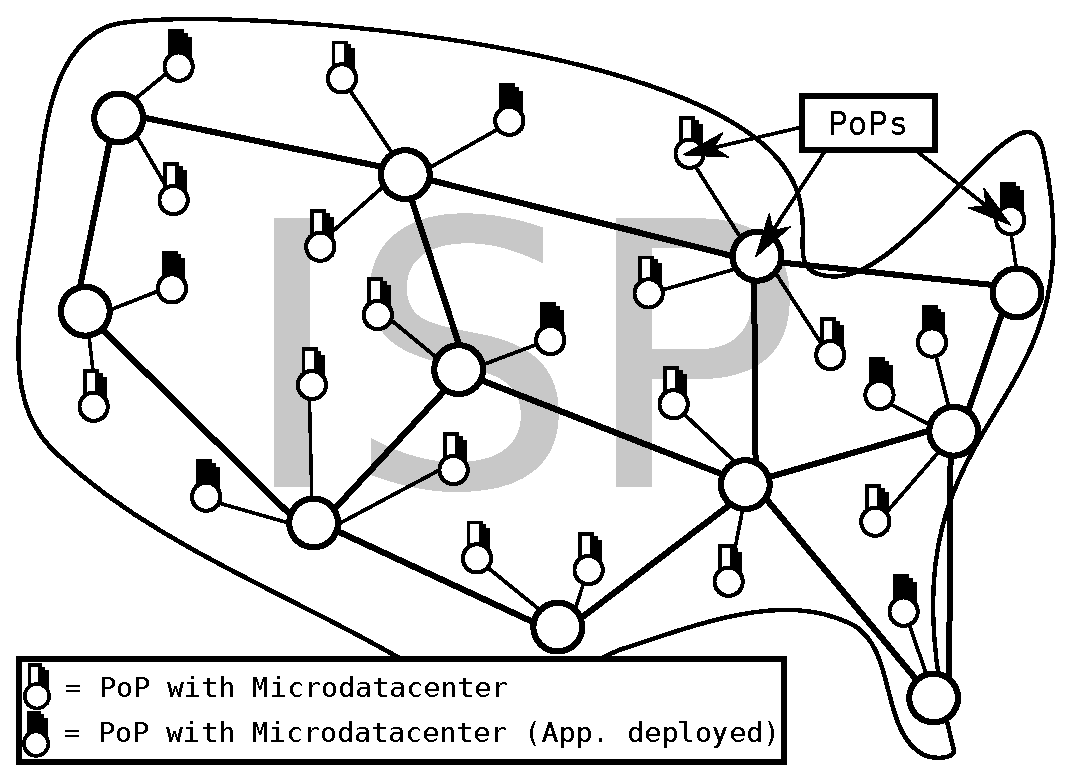
\includegraphics[width=0.9\linewidth]{figures-pdf/ISP+Content} 
\end{center}
\caption{\MDCs in an ISP with \Netpaas enabled} 
\label{fig:story} 
\end{figure}

Figure~\ref{fig:story} illustrates the basic idea. The ISP can offer
\emph{slices} within its microdatacenters, that can be leased by the
CDIs---using our proposed mechanism---based on their needs. This approach
leverages recent advances in virtualization technology, and flexible billing
models, such as pay-as-you-go, to provide cost-efficient and scalable service
deployment, enabling unprecedented flexibility.  Moreover, the diversity of
available service locations within the network can be used to improve end-user
experience and makes it possible to launch even more demanding applications,
such as interactive ones. On-demand service enables CDIs to rely on a fixed
infrastructure deployment for their baseline operation and then scale it up by
dynamically allocating resources closer to end-users. It also lowers the burden
of entrance in the service market for smaller CDIs who might rely exclusively
on the \onservice at first.

\subsubsection{Microdatacenter
Specifications}\label{sec:microdatacenters-specification}

Microdatacenters consist of one or more racks of off-the-shelf hardware
deployed in general purpose rack space at network aggregation points.
State-of-the-art solutions have been proposed by the VMware/Cisco/EMC VCE
consortium \cite{VCE}, and are also offered by other vendors, such as NetApp
and Dell.  These solutions are general-purpose and provide a shared
infrastructure for a large range of applications. They typically consist of two
basic components: hardware and management software.

\begin{description*} \item [Hardware:] Typical microdatacenters include
\emph{storage}, \emph{computing}, \emph{memory}, and \emph{network access}
components.  Storage consists of tens of Terabytes with an ultra-fast
controller providing I/O throughput in the order of hundreds of Gbps. The
storage component is connected to the Internet through multi-Gbps interfaces
and to the computing component with Gigabit Ethernet switches.  Typically, a
rack includes up to 40 physical multi-core blade servers as well as two routers
and two switches in mesh configuration, for redundancy and load balancing.
\item [Management Software:] Each vendor offers a set of management tools not
only for administering the components but also to create resource slices and to
delegate the operation of the slices to external entities. This can be done
per-server or via hardware supported virtualization\footnote{ For example,
para-virtualization~\cite{virtualization} presents the VM with an abstraction
that is similar but not identical to the underlying hardware.}. The management
software is also responsible for storage allocation and handling network
resources, including IP address space. In addition, the management tools come
with a monitoring interface that allows the ISP to monitor the utilization of
the overall microdatacenter as well as the information for each slice that can
be shared with the external entity.  \end{description*}

An ISP can allocate resource slices consisting of computing, storage, memory,
and network access in a microdatacenter and then delegate the operation of the
slice to a CDI. This is what we refer to as the \emph{ISPs cloud service} which
is realized via resource slices in microdatacenters throughout the ISPs
infrastructure.

\subsubsection{Microdatacenter Network Footprint}\label{sec:microdatacenters-footptint}

Most ISPs' networks consist of an access network to provide Internet access to
DSL and/or cable customers, as well as an aggregation network for business
and/or VPN customers. Routers at this level are often referred to as {\em edge
routers}.  The access and aggregation networks are then connected to the ISP's
backbone which consists of {\em core routers}.  {\it Border routers} are core
routers that are used to connect either to other networks or to co-location
centers.  Opportunities to deploy microdatacenters exist at each level: edge,
core, or border router locations.

The advantage of deploying service infrastructure only at the core router
locations is that there are a few large and well established locations. This is
also a disadvantage as location diversity might be limited. Location diversity
is highest at the edge router locations.  However, it might not always be
possible to deploy a microdatacenter, i.e., due to limited space and/or power
at the facilities, or due to cost. These locations, however, minimize the
distance to the customers.  Border router locations are often a subset of core
routers, hence they inherit the same advantages and disadvantages.

The advantage of using an ISP cloud service vs.\ a public cloud
service for a CDI is the chance to minimize the distance to the
end-user. \ondemandbase allows the CDI to control the
location of the slices and ensures that there are no major network
bottlenecks.


\subsection{\OnService Design}\label{sec:service-design}

An {\it \onservice} is a service of the ISP (see Figure~\ref{fig:story}) that
enables CDIs to use a hosting infrastructure that scales according to end-user
demands, so as to minimize its capital expenditures and operating costs, as
well as the distance between its hosting infrastructure and the source of the
demand.  Moreover, it offers an interface that enables the CDI to map user
requests to appropriate slices in order to maximize slice utilization and
minimize the distance between the end-user and the slices.

{\bf Definition 1: ISP \OnService.}  The ISP \onservice is a service offered by
the ISP and uses as its base unit of resource allocation the notion of a
microdatacenter \emph{slice}.  It is the ISP's task to allocate/de-allocate the
slices since it operates the microdatacenter.  The CDI requests slices based on
its clients demand. When the slice is allocated to the CDI, the service can be
installed on the slice. From that point on, the CDI fully controls the
operation of the service installed in the microdatacenter. Negotiation about
slices are done via the \emph{\onservice interface} through which CDI demands
are matched to the ISPs resources. How to map demands to resources in an
efficient manner is the task of the ISP and part of the \emph{\onservice
realization}.  In addition, the interface allows for access to the billing
information.  Moreover, the \emph{\onservice interface} enables the mapping of
user requests to appropriate slices.

The above mentioned use of microdatacenters is in-line with the available
primitives of private and public clouds operated in large-scale datacenters,
\eg~\cite{amazon,azure}.


\subsubsection{Microdatacenter Slice}\label{sec:Slice}

Based on our description of microdatacenters in the previous sections, we define
a slice as follows.

{\bf Definition 2: Slice.} The slice of a microdatacenter is a set of
physical or virtualized resources of a specific capacity, for each of the
resources of the microdatacenter. The slice is delegated to the service
provider that can install and operate its service using the resources of
the slice.

For example, a slice can be a 1-core server with 2 GB RAM, 30 GB storage, a
1 Gbps Internet access bandwidth, 2 public IPs---an actual physical resource.
Alternatively, it can be a VServer with 2GB and 1 Gbps Internet
access bandwidth, 1 public IP, and a pre-installed OS---a virtual machine
of a specific type.  With the current management and virtualization tools
available from microdatacenter vendors, it is possible to
allocate/deallocate slices on-demand in with unprecedented degree of
freedom, \eg~\cite{aboveclouds} and references within.


\subsubsection{\OnService Realization}\label{sec:Realization}

Based on the above specification of \onservice, the ISP has to implement two
functions to offer its \onserviceemph: \emph{mapping of service pro\-vi\-der
demands to slices} and \emph{assigning users to slices}.

Note, the time scales at which these two services are expected to be used
differ significantly. The first one allows the service provider to flexibly
allocate and de-allocate its slices based on its forecast of demands, in those
locations where it wants them.  We foresee that requests for slices are not
issued individually but rather collectively on a time scale of tens of minutes
or hours.

The CDI provides the ISP with a set of demands for slice resources, predicted
demand locations, desired slice locations, as well as optimization criteria.
The ISP then has to map the demands to its microdatacenter resources.  We
expect that the major degree of freedom that the ISP uses to jointly optimize
performance is the desired slice location. We refer to this optimization
problem as the \sliceallocation problem. If the desired slice locations are
fully specified or the predicted demand locations are missing, the
\sliceallocation problem becomes trivial and the ISP only grants or denies the
request.

At the second time scale, the ISP can help the CDI in assigning users to
slices. Since the service is offered at multiple locations, a good assignment
of users to slices impacts not only the load on the network but also the
network delay and packet loss, which are key contributors to the user
experience. Jointly optimizing this mapping is therefore of interest to both
the ISP and the CDI. The CDI can query the ISP for each request on where to map
it, based on the current set of slice assignments and service loads. The ISP
then uses its network information to propose possible slices. We refer to this
problem as the \sliceassignment problem, see \cite{Cate-CCR}.

Another degree of freedom \onservice offers to the CDI is auto-scaling.  While
it is quite feasible to dimension applications, flash-crowds or device failures
are hard to predict. To this end, a CDI may allow \onservice to create replicas
if its monitoring indicates that the capacity of the service at a given
location is or will be exceeded.  To realize this service, the ISP needs to
constantly monitor resource availability and if necessary migrate or suggest
the creation of additional slices. Moreover, it has to allow the CDI to monitor
the utilization of its slices.


\subsubsection{Service Interfaces}\label{sec:service-interfaces}

The ISP offers four interfaces to the content delivery Infrastructures:

\begin{description*}

\item [Resource discovery:] Using this interface the CDI requests information
about resources, e.g., about available locations for slices and if in principle
slices are available at those locations at what price.

\item [Slice allocation:] Using this interface the CDI requests slice
allocation within a certain cost limit.

\item [User-slice assignment:] Using this interface the CDI requests
recommendations for user demand to slice mapping.

\item [Monitoring and billing:] Using this interface the CDI monitors the
status and cost of its slices.

\end{description*}

In Section~\ref{sec:future-netpaas} we give specific examples of how these
service interfaces can be used by a CDI and ISP to cooperate in order to
improve their services.


\subsubsection{Billing}\label{sec:billing}

It is important for the CDI to minimize and track the cost of its use of
\onservice.  Depending on the scale of the services, the service provider has
to pay the usual price or negotiate bilateral agreements with the ISP. Using
the resource discovery interface, it estimates the cost of slice allocation at
possible locations. Using the slice allocation interface, it can bound the
total cost of the request.

We expect that the billing of a slice allocated via \onservice follows that of
large-scale datacenters.  This means that there is an installation cost and a
usage cost.  The installation cost applies to a single slice in a
microdatacenter and is charged only once or over long time intervals, \eg
hours, and is fixed. The installation cost typically increases if additional
licenses have to be leased, \eg software licenses. The installation cost can
depend on the location of the microdatacenter that hosts the slice or the
time-of-day.

The usage cost follows a pay-as-you-go billing model and charges for the usage
of different resources assigned to a slice.  The billing among different
resources in the same slice can be quite diverse. The slice can use expensive
resources such as bandwidth or cheaper ones such as CPU.

For example, a slice may have a $\$ 0.01$ per hour installation cost and a
usage cost that depends on its use of various resources, \eg $\$ 0.02$ per real
CPU usage per hour, $\$ 0.001$ per GByte stored per hour, and $\$ 0.001$ per
Gbps outgoing traffic per hour.  If the slice is idle, then only the
installation cost is charged. Note, that if the slice is used for a short
period within the allocation time, \eg a few minutes, then the charge may apply
to the minimum billing granularity.

To minimize the cost of deploying an on-demand service, the CDI can change its
total slice demands as well as its slice specifications dynamically. Moreover,
it can relax the slice specifications to reduce overall cost of its service
deployment.



\subsection{Network Platform as a Service (NetPaaS)}\label{sec:future-netpaas}

Next, we discuss the prototype system that has been proposed to materialize the
On-demand service, Network Platform as a Service (NetPaaS). NetPaaS leverages
the view of PaDIS and also utilize the knowledge about the status of the
microdatacenters within the network. NetPaaS is also able to map the requests
of CDIs to available microdatacenters to better match the demand with the
resources inside the network.  The granularity at which they are exchanged via
the service interface.  We also outline several possible protocols for the
service interfaces. We focus on resource discovery, slice allocation, and
user-slice assignment. We do not discuss monitoring and billing because they
can be realized today using techniques similar to those in use by current
public clouds, \eg~\cite{aboveclouds}. Due to space limitations, we refer the
reader to \cite{NetPaaS} for a formalization of NetPaaS, as well as an
evaluation on a CDI use case.

Recall that our assumption that the time scales at which the two principle
components of \onservice operate are different. On the one hand, resource
discovery and slice allocation are expected to be done on time scales of tens
of minutes, hours, or even days. On the other hand, user-slice assignment
potentially happens on a per user request basis. Accordingly, the protocols
differ. We propose to use out-of-band protocols for the first two service
interfaces and in-band protocols for the third one.


\subsubsection{Resource Discovery}\label{sec:Resource-Discovery}

The purpose of resource discovery is to provide the CDI with the ability to
gather information about the resources offered by the ISP. Accordingly, we
have two message types: CDI\_Discovery\_Request and ISP\_Discovery\_Re\-sponse.

\begin{description*}

\item [CDI\_Discovery\_Request:] Is issued either without and with arguments.
In the first case the response is the set of resources that are offered. In the
second case the responds contains details about the resources named in the
argument.

\item [ISP\_Discovery\_Response:] List of available resource or details about
the resources specified in the argument.

\end{description*}

So far we have not outlined at what granularity and specificity the resources
are requested. This depends on the agreements between the CDI and the ISP.  For
example, the ISP may have no problem revealing its microdatacenter locations to
a major CDI. However, it may not want to share this information with an
untrusted CDI that wants to run a single slice. For the latter, the region in
which the microdatacenter is located might well suffice.

With regards to granularity, the ISP can specify which type of servers it is
offering in each microdatacenter region, as is common for public cloud
services~\cite{amazon}, unless another agreement is in place that enables
access to more specific information.  With regards to the availability and/or
price, the ISP can either return a base price, including installation and usage
cost, to indicate that resources are available or offer an auction-based
system. In the latter case, the discovery request returns information about
past prices.

\subsubsection{Slice Allocation}\label{sec:system-slice-allocation}

\begin{figure}
    \begin{center}
    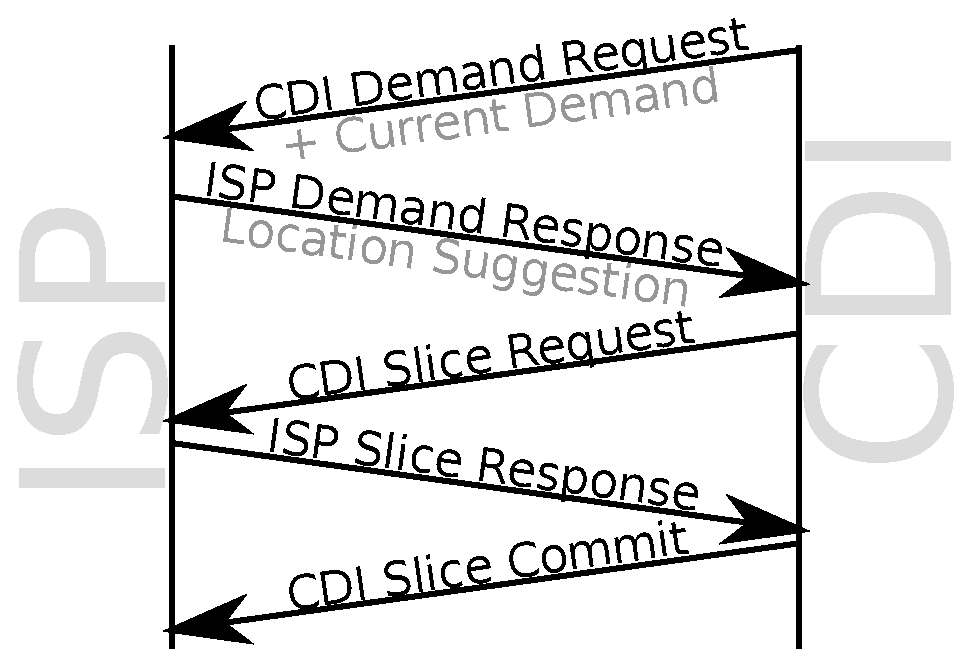
\includegraphics[width=0.6\linewidth]{figures-pdf/Resource_Negotiation}
    \end{center}
    \vspace*{-1em}
    \caption{Slice allocation message exchange.}
    \label{fig:ResourceAllocation}
\end{figure}

Slice allocation enables the CDI and ISP to cooperate for allocating slices in
microdatacenters close to the end-user that are able to satisfy the demands.
We envision five message types: CDI\_Demand\_Request, ISP\_Demand\_Response,
CDI\_ Slice\_Request, ISP\_Slice\_Response, CDI\_Slice\_Commit. The first two
message types enable the cooperation between the CDI and the ISP to allocate
slices at appropriate microdatacenter by utilizing network information, see
Figure~\ref{fig:ResourceAllocation}. The last three messages enable a three way
handshake between the CDI and the ISP to verify that the ISP is able to provide
a specific slice for the CDI.

\begin{description*}

\item [CDI\_Demand\_Request:] Is submitted by the CDI to the ISP and contains a
summary of the hardware resources the CDI wants together with optimization
criteria, constraints, and a demand forecast, \eg per region or per network
prefix.  Possible optimization criteria are to minimize network distance or the
cost. The constrains include: number of locations, minimum resources per slice,
etc.

\item [ISP\_Demand\_Response:] The ISP returns a set of proposed slice
configurations and their price. It computes these by solving the
\sliceallocation problem.

\item [CDI\_Slice\_Request:] The CDI either selects, based on its criteria, a
set of proposed slices as returned by the ISP\_De\-mand\_Response, or it
completes a specification of a slice set request using information it retrieved
via the resource discovery interface. In addition, the request contains a
maximum cost.

\item [ISP\_Slice\_Response:] Upon receiving a CDI\_Slice\_Request, the ISP
checks if it can offer the set of slices at the requested cost. This involves
solving another version of the \sliceallocation problem. If possible, the ISP
returns the price otherwise it declines the request.  At this step, the ISP
reserves the requested resources to guarantee their availability. Note, the ISP
does not have to return precise slice definitions, \eg instead of returning
that slice x should be located in microdatacenter~y attached to router~z it
only returns slice~x should be located in region~xyz.

\item [CDI\_Slice\_Commit:] This step confirms CDI\_Slice\_Requests. Upon
receiving the commit from the CDI, the ISP allocates the slices and delegates
their control to the CDI.  

\end{description*}

Now we discuss different ways in which a CDI and an ISP can cooperate using the
above messages. These ways differ in which information is shared and with whom.

\begin{description*}

\item [Minimum information exchange:] The CDI uses the information from the
ISP\_Demand\_Response for queries via CDI\_Demand\_Request with a uniform
distributed demand vector. The responses include slice candidates with servers
having specified hardware profiles and in specific regions. Then, the CDI
scales the suggested slices according to its demand locations and uses the
CDI\_Slice\_Request message to check if the ISP can offer it and at what price.
Once it has found a satisfactory configuration it can use the
CDI\_Slice\_Commit message to request the necessary slices.


\item [Partnership 1:] The CDI uses CDI\_Demand\_Request with a scaled demand
CDI selects one of these and uses the ISP\_Slice\_Request message so that the
ISP can reserve the resources. Upon successful reservation, the
CDI\_Slice\_Commit message confirms the allocation of the slices.

\item [Partnership 2:] The CDI uses the CDI\_Demand\_Request without a demand
vector but with specific resource requests. The ISP response specifies
candidate microdatacenters with available resources.  Then, the CDI uses its
version of the \sliceallocation problem to find possible slice sets at a subset
of these locations. Then, the CDI uses the ISP\_Slice\_Request message to see
if the ISP can offer it and at what price. Once it finds a satisfactory
configuration it uses the CDI\_Slice\_Commit message to allocate the slices.

\end{description*}

The first scenario corresponds to the minimum information that has to be
exchanged in order to reach a consensus on the locations and specification of
the slices. The latter two summarize different forms of possible cooperations
that can be agreed upon in bilateral agreements.

So far, we have assumed that there are no preallocated slices. However, this is
typically not the case, and the actual task is to augment a preexisting set of
slices in such a way as to best serve the predicted demand for the next time
period. To enable this, another argument to each message request can be
provided, indicating a set of already allocated resources and a penalty value
for deallocating slices in one location and allocating them in another.  This
penalty is needed as part of the optimization problem.  Basically, it indicates
up to which point it is preferable to keep a suboptimal location because of
stability of resource allocation vs.\ when to migrate the service to a new
location.  Based on the returned information, the CDI has the option of either
moving slices using VM migration or to de-allocate and allocate new slices.

The ISP microdatacenter can offer VM migration and/or
consolidation\footnote{Here, consolidation corresponds to moving multiple VMs
with minimal resource requirements to the same physical machine to keep a base
service.} with keeping the IP addresses only within the same microdatacenter
location. Across microdatacenters it may only offer migration with tunnels
which requires the CDI to temporarily operate two slices at both locations.
However, the old one is a good candidate for consolidation so that it is
possible to reduce the allocated resources to a minimum within a
microdatacenter once all new requests are served by the newly allocated slices.
Thus, if an ISP offers service consolidation, one option for CDIs that want to
use diverse sets of microdatacenters is to always keep a minimal slice active
at each location and expand or shrink it according to the demand.

\subsubsection{User-Slice Assignment}\label{sec:system-user-assignment}

\begin{figure}[tbp]
    \begin{center}
    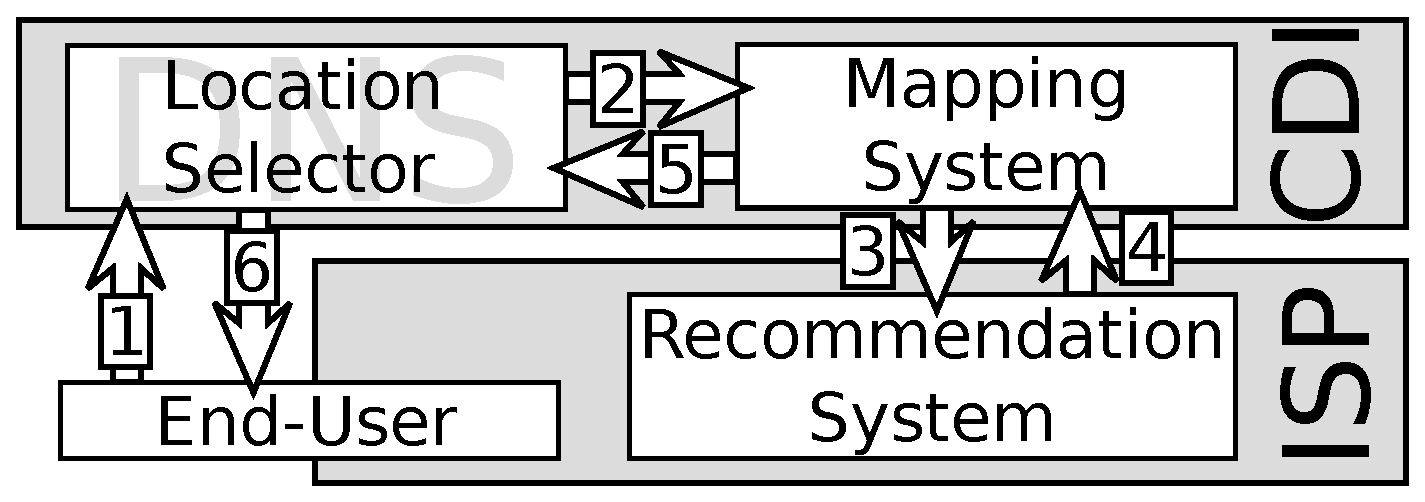
\includegraphics[width=0.8\linewidth]{figures-pdf/Mapping_System}
    \end{center}
    \vspace*{-1em}
    \caption{User-slice assignment schematic.}
    \label{fig:UserSliceAllocation}
\end{figure}

The purpose of the user-slice assignment interface is to enable small time
scale interactions between the CDI and the ISP, to ensure that end-user demand
is mapped to the appropriate slice.  Therefore, the interface has to be
integrated into the process used by the CDI to map user requests to CDI
servers.  Next, we first review how this is currently realized using DNS. Then,
we discuss options on how the user-slice assignment interface can be
integrated, see Figure~\ref{fig:UserSliceAllocation}.

{\bf CDI: User request to CDI server mapping.} Before an end-user issues a
request for the CDI service, \eg downloading some content or watching a video,
it issues a DNS request to map the hostname to an IP address of the server that
hosts the service.  This DNS request is sent to the ISPs DNS resolver or an
alternative DNS resolver. This resolver contacts the authoritative DNS server
of the CDI service, since caching is typically restricted by small TTL's. The
authoritative DNS server uses a CDI service, the CDI mapping system, to select
a CDI server from which to satisfy the future requests of this end-user. The
CDI mapping system performs a CDI specific optimization.  This optimization may
consider the load on the CDI servers, the network location of the CDI server as
well as the requesting DNS server, the price of network access at the CDI
server, etc. Note, the CDI's authoritative DNS name servers usually does not
have access to the IP address of the end-user as the request is forwarded via
the DNS resolver unless the eDNS~\cite{DNS-extension-IP-client} standard is
used.  With eDNS, the client IP address or the IP prefix can be added to the
DNS request sent by the DNS resolver to the authoritative DNS name server. In
addition, the CDI can use HTTP redirection to further load balance within its
infrastructure.


{\bf User-Slice Assignment: Option 1.} Considering the process outlined above,
one possible way to use the user-slice assignment interface is within the
optimization that the CDI mapping system performs.  For this case, we envision
two message types: CDI\_User-Slice\_Assign\_Re\-quest and
ICDI\_User-Slice\_Assign\_Response which correspond to steps 3 and 4 in
Figure~\ref{fig:UserSliceAllocation}.


\begin{description*}

\item [CDI\_User-Slice\_Assign\_Request:] Issued by the CDI's DNS server to the
  ISP. It contains the client IP address as well as slice locations within or
  outside of the ISP.

\item [ISP\_User-Slice\_Assign\_Response:] The ISP responses with a ranking of
  the slice locations.

\end{description*}

The previous two messages enable the CDI to consider information from the ISP,
conveyed via the ranking, for its mapping. This is equivalent to the
functionality and protocols proposed by the IETF ALTO working group.  However,
we envision a more light weight implementation. We propose to not rely on XML
for encoding each request if the granularity of the requests is on a per
connection level. If the CDI uses a coarser granularity such as subnet or
region, the efficiency of the message exchange is even less critical.\\

{\bf User-Slice Assignment: Option 2.}
Another way to integrate the user-slice assignment interface within
the above process is by pro-actively sharing information between the CDI
and the ISP.  For this case, we again envision two message types:
ISP\_User-Slice\_Assign\_Pro\-po\-sal and CDI\_User-Slice\_Assign\_Ack.

\begin{description*}

\item [ISP\_User-Slice\_Assign\_Proposal:] Is sent by the ISP to the CDI
  mapping system. It contains a set of IP prefixes each with an associated
  ranking of the different microdatacenter locations.

\item [CDI\_User-Slice\_Assign\_Ack:] The CDI either acknowledges or rejects
  the proposal.

\end{description*}

This again enables the CDI to include information from the ISP, conveyed via
the ranking, in its mapping.  For example, one can use BGP to send such
messages---a mechanism Akamai already utilizes to aid in mapping users to
its clusters~\cite{Akamai-Network}.


\subsection{Summary}

Motivated by the high requirements newly deployed services put on the ISPs
networks, we formally introduced the design of on-demand services to relieve
both the CDI and the ISP.  We also provided the design and implementation of
\Netpaas, a system to orchestrate the deployment of on-demand services using
the ISPs view of the network and available resources. In~\cite{NetPaaS} we
evaluate \Netpaas using operational traces from the biggest commercial CDN and
a European Tier-1 ISP. We quantify the benefits of \Netpaas by utilizing
different optimization goals \eg delay reduction or reduced link utilization.
Our results show that \Netpaas yields encouraging results for a joint
deployment of new services that significantly improves the end-users
performance while reducing the network utilization for the ISP and offering
agile service deployment to the CDI. For the analysis and performance evaluation of
on-demand server placement algorithms in wide-area networks we refer the reader
to~\cite{ToN-dFL} and \cite{SimultaneousSourceLocation}.

